\documentclass[12pt,a4paper]{article}
\usepackage[utf8]{inputenc}
\usepackage[english,russian]{babel}
\usepackage{amssymb,amsfonts,amsmath,cite,enumerate,float,indentfirst}
\usepackage{graphicx}
\usepackage{geometry}
\usepackage{systeme}
\usepackage{hyperref}
\usepackage{url}
\hypersetup{
	colorlinks,
	citecolor=black,
	filecolor=black,
	linkcolor=black,
	urlcolor=black
}
\geometry{left=2cm}
\geometry{right=1.5cm}
\geometry{top=2cm}
\geometry{bottom=2cm}

\newcommand\Set[2]{\{\,#1\mid#2\,\}}
\newcommand{\floor}[1]{\lfloor #1 \rfloor}

\begin{document}
	
\begin{titlepage}
	\begin{center}		
		\vfill	
		Санкт-Петербургский политехнический университет \\
		Петра Великого\\
		\vskip 1cm
		Институт прикладной математики и механики \\
		Кафедра «Прикладная математика»
		\vfill
		\textbf{Отчёт\\
			по лабораторной работе №1\\
			по дисциплине\\
			«Математическая статистика»\\}
		\vfill
	\end{center}
	\vfill
	\hfill
	\begin{minipage}{0.4\textwidth}
		Выполнил студент:\\
		Шагвалиев Михаил Александрович\\
		группа: 3630102/80201\\
	\end{minipage}
	\vfill
	\hfill 
	\begin{minipage}{0.4\textwidth}
		Проверил:\\
		к.ф.-м.н., доцент\\
		Баженов Александр Николаевич\
	\end{minipage}
	\vfill
	\begin{center}
		Санкт-Петербург\\2020 г.
	\end{center}
\end{titlepage}

\tableofcontents
\pagebreak
\listoffigures
\pagebreak

\section{Постановка задачи}
Для 5 распределений:

\begin{itemize}
	\item Нормальное распределение $N(x, 0, 1)$
	\item Распределение Коши $C(x, 0, 1)$
	\item Распределение Лапласа $L(x, 0, \frac{1}{\sqrt{2}})$
	\item Распределение Пуассона $P(k, 10)$
	\item Равномерное распределение $U(x, -\sqrt{3}, \sqrt{3})$	
\end{itemize}

Требуется сгенерировать выборки размером 10, 50 и 1000 элементов, построить на одном рисунке гистограмму и график плотности распределения.

\pagebreak

\section{Теория}
\subsection{Рассматриваемые распределения}
Плотности:

\begin{itemize}
	\item Нормальное распределение 
	\begin{equation}
	N(x, 0, 1)=\frac{1}{\sqrt{2\pi}}e^{-\frac{x^2}{2}}
	\end{equation}
	
	\item Распределение Коши
	\begin{equation}
	C(x, 0, 1)=\frac{1}{\pi(x^2+1)}
	\end{equation}
	
	\item Распределение Лапласа
	\begin{equation}
	L(x, 0, \frac{1}{\sqrt{2}})=\frac{1}{\sqrt{2}}e^{-\sqrt{2}|x|}
	\end{equation}
	
	\item Распределение Пуассона
	\begin{equation}
	P(k, 10)=\frac{10^k}{k!}e^{-10}
	\end{equation} 
	
	\item Равномерное распределение
	\begin{equation}
	U(x, -\sqrt{3}, \sqrt{3}) =
	\begin{cases}
	\frac{1}{2\sqrt{3}} & |x| \leq \sqrt{3} \\
	0 & |x|>\sqrt{3}
	\end{cases}
	\end{equation}	
\end{itemize}

\subsection{Гистограмма}
В математической статистике гистрограмма — это функция, приближающая плотность вероятности некоторого распределения, построенная на основе выборки из него. \cite{Histogram}

\subsubsection{Построение гистограммы}
Пусть $X = \{x_1,...,x_n\}$ — выборка, $[a,b]$ — отрезок, на котором строится гистрограмма 
\begin{enumerate}
    \item $[a,b]$ разбивается на $m$ равных интервалов:
    \begin{equation}
        \Delta_i = (a+\frac{i-1}{m}(b-a), a+\frac{i}{m}(b-a)), i \in \{1,...,m\}
    \end{equation}
    
    \item Подсчитаем количество элементов выборки, попавших в интервал $\Delta_i$:
    \begin{equation}
        d_i =|\Set{k}{x_k\in\Delta_i}|, i \in \{1,...,m\}
    \end{equation}
    
    \item Построим прямоугольники с основанием $\Delta_i$ и высотой $\frac{d_i}{c}$, где $c$ — общее число элементов выборки, попавших в $[a,b]$ (таким образом, гистрограмма "отнормирована": сумма площадей всех прямоугольников равняется единице).
\end{enumerate}

В качестве $(a, b, m)$ возьмем, соответственно, $(\min_{x \in X} x, \max_{x \in X} x, \floor{3\sqrt[3]{n}})$ 

\pagebreak

\section{Реализация}
Работа выполнена с помощью языка \textbf{Python} в IDE \textbf{PyCharm}, также были использованы библиотеки:

\begin{itemize}
	\item \textbf{scipy} - генерация данных
	\item \textbf{numpy} - работа с массивами
	\item \textbf{matplotlib} - отрисовка графиков
\end{itemize}

Исходный код работы приведен в приложении.
\pagebreak

\section{Результаты}
\subsection{Гистограммы и графики}
\begin{figure}[h!]
	\centering
	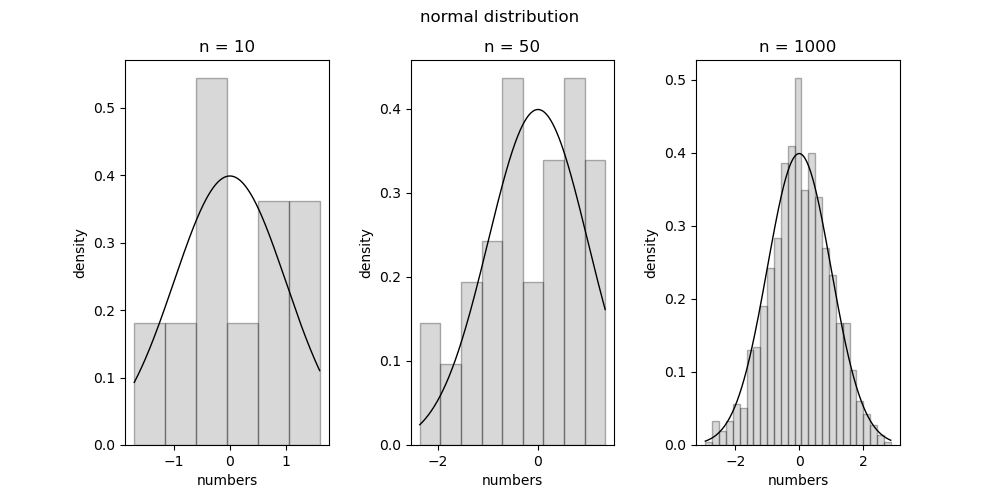
\includegraphics[scale=0.7]{normal.png}
	\caption{Нормальное распределение}
	\label{fig:image}
\end{figure}

\begin{figure}[h!]
	\centering
	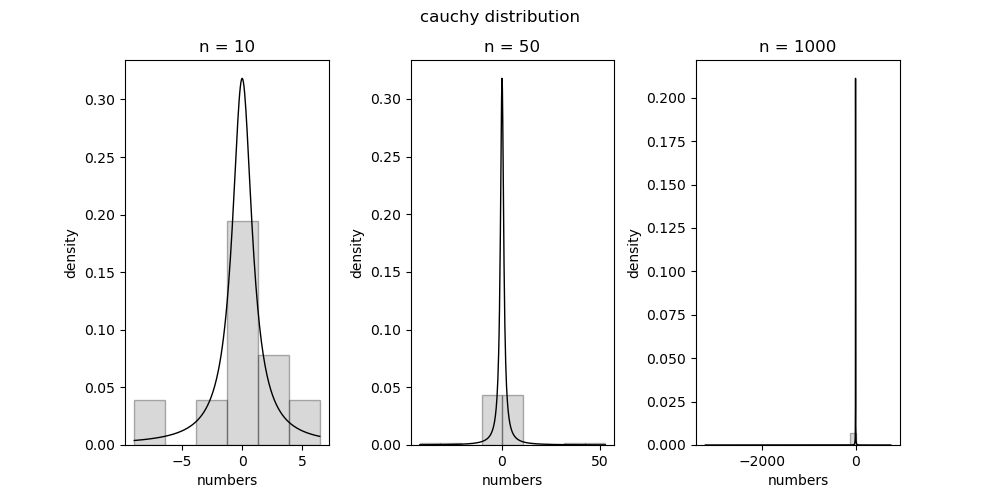
\includegraphics[scale=0.7]{cauchy.png}
	\caption{Распределение Коши}
	\label{fig:image}
\end{figure}

\pagebreak

\begin{figure}[h!]
	\centering
	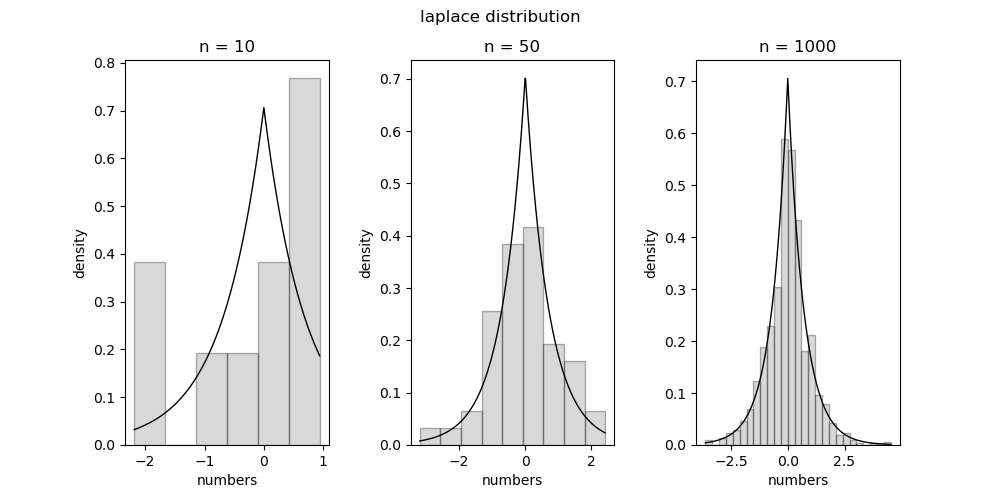
\includegraphics[scale=0.7]{laplace.png}
	\caption{Распределение Лапласа}
	\label{fig:image}
\end{figure}

\begin{figure}[h!]
	\centering
	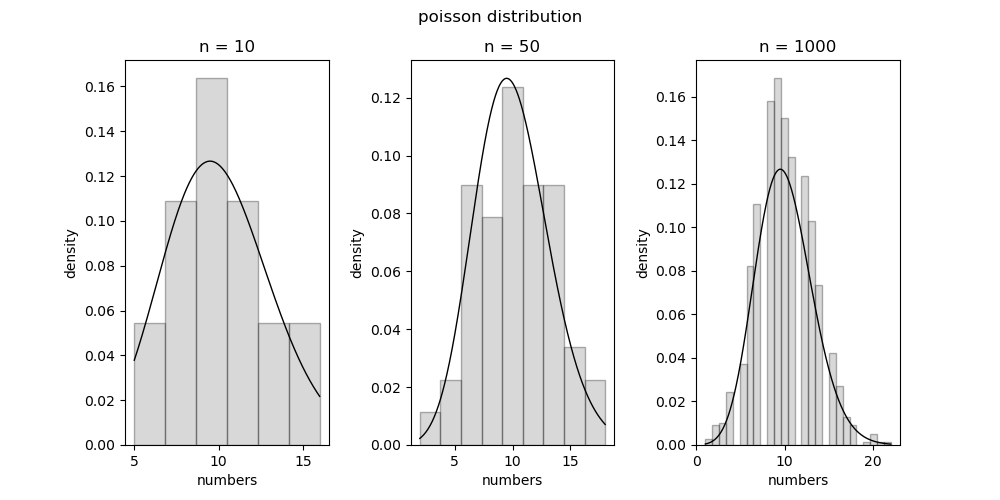
\includegraphics[scale=0.7]{poisson.png}
	\caption{Распределение Пуассона}
	\label{fig:image}
\end{figure}

\pagebreak

\begin{figure}[h!]
	\centering
	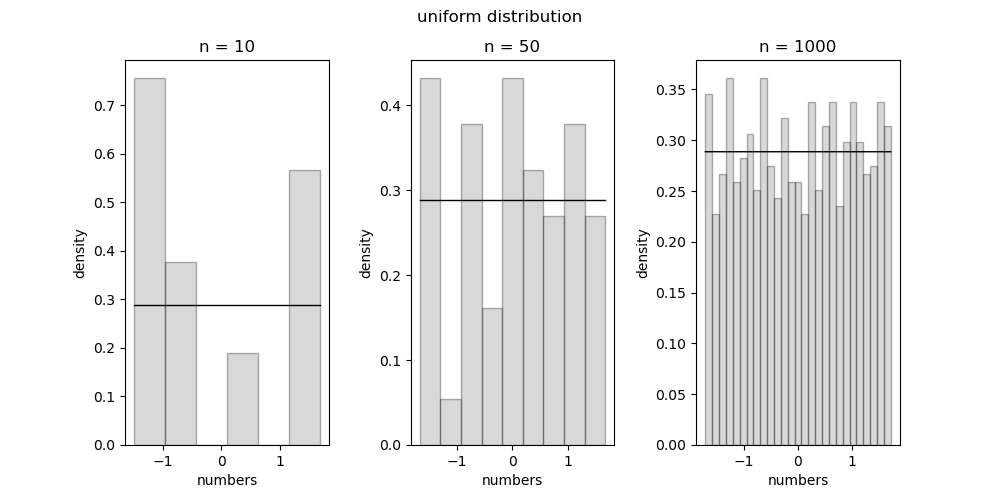
\includegraphics[scale=0.7]{uniform.png}
	\caption{Равномерное распределение}
	\label{fig:image}
\end{figure}
\pagebreak

\section{Обсуждение}
По результатам проведенной работы можно сделать вывод о том, что чем больше выборка, тем лучше гистрограмма приближает функцию плотности распределения случайной величины. Чем меньше выборка — тем хуже по гистограмме определяется распределение случайной величины.
\pagebreak

\section{Приложения}
\noindent 1. Код лабораторной: {\url{https://github.com/MekhailS/math-statistics-labs/tree/master/lab1_histogram}}

\begin{thebibliography}{9} 
	\addcontentsline{toc}{section}{Список литературы}
	\bibitem{Histogram} Histogram. URL: {\url{https://en.wikipedia.org/wiki/Histogram}}
\end{thebibliography}

\end{document}
